\section{Introduction}

\subsection{Objectives} 

\begin{itemize}
\item Learn basic facts about the Karel language and its history. 
\item Learn how Karel differs from other programming languages.
\item Learn what skills this course provides.
\end{itemize}

\subsection{Brief history}

The educational programming language Karel the Robot was introduced by Richard E. 
Pattis in his book "Karel The Robot: A Gentle Introduction to the Art of Programming" in 1981. 
Pattis first used the language in his courses at Stanford University, and now it is used at 
countless schools in the world to introduce students to algorithmic design and computer programming. 
The language is named after Karel \v{C}apek, a Czech writer who invented the word "robot" in his 1921 
science fiction play R.U.R. (Rossum's Universal Robots).

\subsection{Who is Karel?}

Karel is a little robot that lives in a maze and loves to collect gems.
He was manufactured with only five simple commands in his memory:
\begin{itemize}
\item {\color{blue} \tt go} ... make one step forward.
\item {\color{blue} \tt get} ... pick up a gem from the ground. 
\item {\color{blue} \tt left} ... turn to the left.
\item {\color{blue} \tt right} ... turn to the right. 
\item {\color{blue} \tt put} ... put a gem on the ground. 
\end{itemize}
He also has five built-in sensors that allow him to check his immediate surroundings:
\begin{itemize}
\item {\color{blue} \tt wall} ... true if he would crash into a wall by making one more step, false otherwise. 
\item {\color{blue} \tt gem} ... true if he stands on a gem, false otherwise.
\item {\color{blue} \tt north} ... true if he is facing North, false otherwise.
\item {\color{blue} \tt home} ... true if he is at home, false otherwise.
\item {\color{blue} \tt empty} ... true if his bag with gems is empty, false otherwise. 
\end{itemize}

\subsection{What does this course have to offer?}

Computer programming skills are highly valued today, and they will be even more 
valued in the future. Karel's language is so natural that we will be able to 
focus on designing great algorithms. This is the most important skill in 
computer programming. In other words, we could start learning programming 
with a technically 
complicated conventional programming language as well, but we would spend lots of time 
battling technical problems. The advantage of starting with Karel is that 
when moving on to other languages, we will be able to focus on the technical 
differences, as the programming concepts we will already understand.


\subsection{Is Karel a toy language?}

{\em Definitely not!} Despite its playful appearance, Karel features all elements 
of modern procedural programming. The complexity of algorithms 
that we will encounter in this course ranges from {\em extremely simple} 
to {\em extremely tough}. Towards the end of this course we will encounter 
tasks that will make our head spin. However, Karel is very light on 
technicalities, which is very good for someone who is just starting out.

The biggest conceptual difference between Karel and standard procedural
programming languages such as Python, C, C++ or Fortran is that {\em the robot does not 
know math}. At least not until we get to advanced levels that are beyond 
the original Pattis' book. In the basic course, we will solve many exercises 
whose objective is to teach how to design great algorithms, and math is 
not needed for that. After finishing this tutorial, we will be able to transition 
smoothly to Python where we can do as much math as we like!
 
\section{Launching Karel}

\subsection{Objectives} 
\begin{itemize}
\item Learn to launch Karel and work with the graphical application.
\item Learn that Karel has several modes and how they differ from each other.
\end{itemize}
\noindent
The simplest way to launch Karel is to click on the icon 
{\em Programming} and select {\em Karel} in the menu. This will launch the application 
in {\em Programming mode} with a randomly generated maze, as shown in Fig. \ref{fig:init}.

\begin{figure}[!ht]
\begin{center}
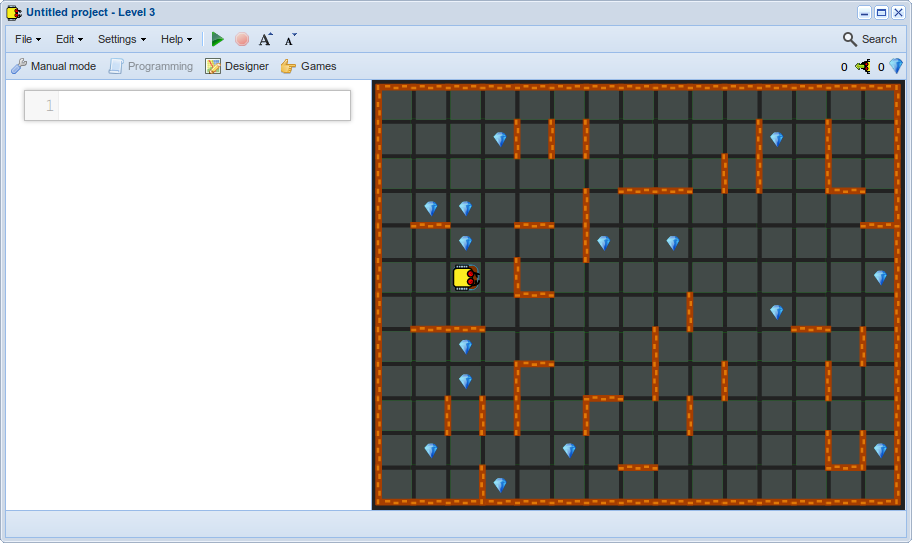
\includegraphics[width=0.7\textwidth]{imgk/init.png}
\end{center}
\vspace{-2mm}
\caption{Launching Karel in Programming mode, with a random maze.}
\label{fig:init}
\vspace{-10mm}
\end{figure}
\newpage
\noindent
The Programming mode is the most frequently used one. It is possible to 
switch to {\em Manual mode}, {\em Designer}, and {\em Games} in the menu. 
These modes will be discussed in Paragraph \ref{levels}.

The application window contains two lines of menus and information on top,
work area on the left, maze on the right, and status bar on the bottom.
The menus are fairly intuitive, so let us just explain a few selected 
functions, starting with the {\em File} menu:

\begin{itemize}
\item {\em Open} will open a file in your account.
\item {\em New} will generate a new random maze.
\item {\em Clone} will copy a Displayed Project into your account. 
\item {\em Display} will submit a project for review. If you think that 
      other users would find your program or game interesting, this is the way to make it 
      available to them. Upon passing the review, the project will be added to Displayed Projects.
\end{itemize}
{\em Edit} menu enables operation with code and text cells (to be discussed in 
Section \ref{sec:editmenu}). In {\em Settings} one can change Karel's {\em Level} (to be discussed
in Paragraph \ref{levels}), change his speed, and adjust sound preferences. The green and red 
buttons are used to run and stop programs, respectively, and the two buttons next to them on
the right can be used to increase and decrease font size. The pair of icons on far right is the 
step counter (that can be reset by clicking on it) and gem counter that indicates how many gems 
Karel has in his bag.

\subsection{Karel modes} \label{levels}

Karel operates in four modes:
\begin{itemize}
\item {\em Manual mode:} The robot is controlled using the mouse and five buttons Go, Get, Left, Right, and Put. 
      Watch out and do not crash!
\item {\em Programming mode:} The robot is controlled using written programs (computer code). The Programming mode is 
      split into several Levels:
\begin{itemize}
\item Level 1 is a transition layer between the Manual and Programming modes. Programs are written using only 
      five commands {\tt go}, {\tt get}, {\tt left}, {\tt right}, and {\tt put} that exactly correspond to 
      the buttons Go, Get, Left, Right, and Put in Manual mode.
\item Level 2 is where the actual programming begins. On top of the commands from Level 1, programs can contain 
      conditions, loops, and custom commands.
\item In Level 3 Karel has a GPS device, and he is able to work with variables and lists. Functions
      can return results.
\end{itemize}
\item {\em Designer:} This mode allows the user to create custom mazes.
\item {\em Games:} Makes it possible to create and play games. 
\end{itemize}

%%%%%%%%%%%%%%%%%%%%%%%%%%%%%%%%%%%%%%%%%%%%%%%%%%%%%%%%%%%%%%%%%%%%%%%%%%%%%%%

\section{Manual Mode} \label{sec:manual}

\subsection{Objectives} 
\begin{itemize}
\item Learn to operate the robot in Manual mode.
\end{itemize}
\noindent
Before we begin, let us review the four directions on the compass:\\[-7mm]

\begin{figure}[!ht]
\begin{center}
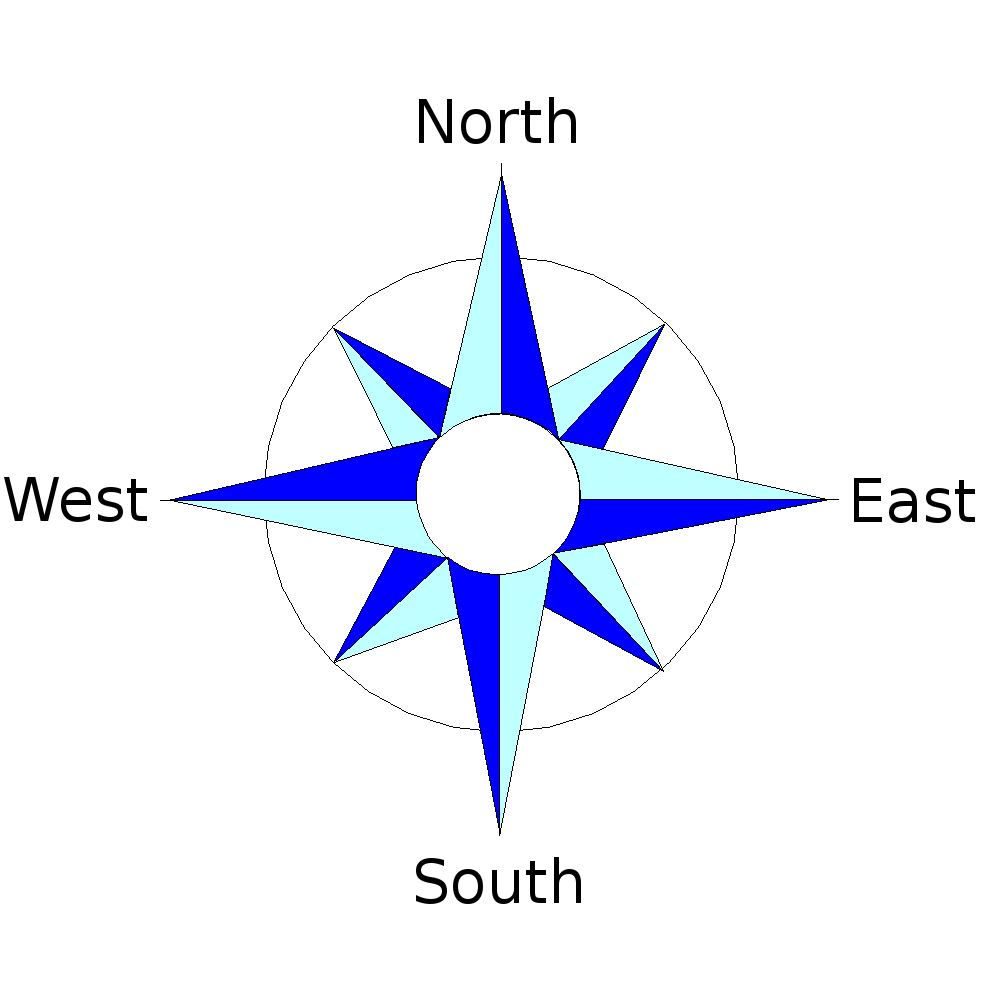
\includegraphics[width=0.35\textwidth]{imgk/compass.png}
\vspace{-0mm}
%\caption{Karel's four possible orientations.}
%\label{fig:ori}
\end{center}
\vspace{-1cm}
\end{figure}

\noindent
When launching Karel through the Programming icon, switch to Manual mode using the corresponding 
menu button. Then, five buttons Left, Right, Go, Get and Put will appear in the panel on the left,
as shown in Fig. \ref{fig:buttons}.

\begin{figure}[!ht]
\begin{center}
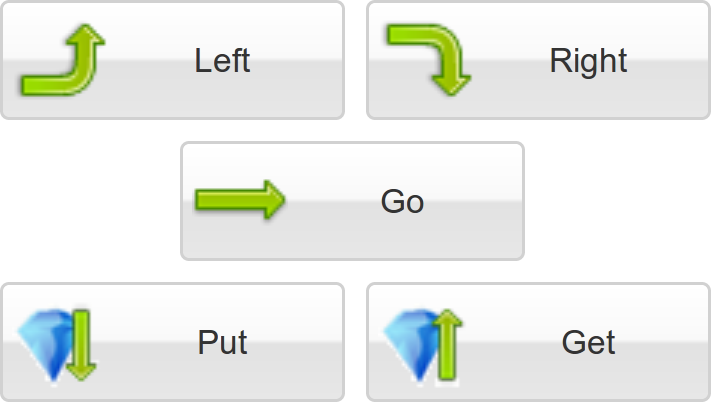
\includegraphics[width=6.2cm]{imgk/buttons-all.png}
\vspace{-0mm}
\caption{Karel's buttons in Manual mode (robot facing East).}
%\vspace{-1cm}
\label{fig:buttons}
\end{center}
\end{figure}
\noindent
The function of the buttons is self-explanatory -- pressing Left will turn the robot 90 degrees to the left,
pressing Right will turn him 90 degrees to the right, and pressing Go will move him one step forward 
(watch out and do not crash!). Upon pressing Put the robot will reach into his bag with gems, 
take one, and put it on the ground where he stands. 
An indicator showing how many gems are in the bag can be found in the upper right 
corner of the window. Last, upon pressing 
Get the robot will pick up a gem from the ground where he stands. If 
one asks the robot to get a gem where there is none, he will complain.

When the robot turns, the arrows on the buttons adjust automatically to his new 
direction. This is illustrated in Fig. \ref{fig:buttons2}.

\begin{figure}[!ht]
\begin{center}
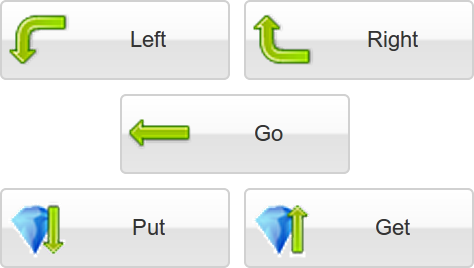
\includegraphics[width=6.2cm]{imgk/buttons-all-2.png}
\vspace{-0mm}
\caption{Karel's buttons in Manual mode (robot facing West).}
\label{fig:buttons2}
\end{center}
\end{figure}

%%%%%%%%%%%%%%%%%%%%%%%%%%%%%%%%%%%%%%%%%%%%%%%%%%%%%%%%%%%%%%%%%%%%%%%%%%%%%%%

\section{Programming Mode} \label{sec:bridge}

\subsection{Objectives} 
 
\begin{itemize}
\item Start operating the robot in Programming mode.
\item Understand the difference between {\em algorithm} and {\em program}. 
\item Learn the difference between {\em syntactical} and {\em logical} mistakes.
\item Understand that {\em debugging} is an indivisible part of computer programming.
\end{itemize}

\subsection{Typing commands}
In Programming mode, commands for the robot are entered into an code cell located in the left panel.
These commands are {\tt left}, {\tt right}, {\tt go}, {\tt get}, and {\tt put}.
Their function is the same as the function of the corresponding buttons in Manual mode.
One or more commands form a {\em computer program (computer code)}. Often 
we just say {\em program} or {\em code}.
There are two simple rules to remember:
\begin{enumerate}
\item Always type one command per line.
\item Do not enter empty characters in front of commands. 
\end{enumerate}
Ignoring these rules would not make the program invalid, but the code would be 
difficult to read. It is important to write a clean, transparent code. 

\subsection{Algorithms, programs, and bugs} \label{subsec:interm1}

Karel always obeys all commands {\em exactly}. Sometimes it may happen that 
we plan one thing but to our surprise the robot does something else. In most cases this 
happens when our {\em algorithm} is wrong. By an {\em algorithm} we mean a sequence of 
logical steps that the robot needs to follow in order to fulfill his task. Algorithms 
are presented using normal human language, not in terms of the robot's commands. 

{\em Program} or {\em computer code} is created when the algorithm is expressed
in terms of the robot's language. When our algorithm is good, then 
the program is easy to write.

Mistakes in algorithms are called {\em logical errors}. A logical error is, for 
example, when we crash the robot into a wall because we forgot to make a turn.
Mistakes such as mis-spelling a command, writing "1o" instead of "10", or forgetting 
indentation are related to 
{\em syntax} and they are called {\em syntactical errors}. Of these two types, 
logical errors are usually much more difficult to find. 

In general, mistakes or either kind are called {\em bugs} and the procedure of 
eliminating them is called {\em debugging}. Depending on how careful we 
were while preparing our algorithm and writing the program, debugging takes either 
a short time or a long time. It does not happen often that a program works correctly
right away. 

When we commit a syntactical error,
the robot will write an error message and do nothing.
If our algorithm contains a logical error, then he will
write an error message and stop executing the program. 
The most usual logical error are:

\begin{itemize}
\item Karel crashes into a wall.
\item The robot tries to collect a gem where is none.
\item He attempts to put a gem on the ground while his bag is empty.
\end{itemize}

%%%%%%%%%%%%%%%%%%%%%%%%%%%%%%%%%%%%%%%%%%%%%%%%%%%%%%%%%%%%%%%%%%%%%%%%%%%%%%%

\section{Counting Loop} \label{sec:repeat}

\subsection{Objectives} 

\begin{itemize}
\item Learn to make the robot repeat something a given number of times.
\end{itemize}

\noindent
In Section \ref{sec:bridge} we successfully crossed the bridge between manual control 
and programming. The bridge collapsed, there is no way back. But do 
not worry about that! The land of Programming is much more beautiful,
and once you understand its beauty, you will never want to leave.

\subsection{The {\tt repeat} command}

The {\em counting loop}, represented by the {\tt repeat} command, can save 
us lots of writing when something is repeated a given number of times. 
For example, for Karel to make 15 steps forward we could type:

\begin{bluecode}
go
go
go
go
go
go
go
go
go
go
go
go
go
go
go
\end{bluecode}
But this is neither efficient nor elegant. Instead, the same can be
achieved by telling Karel to {\tt repeat} the {\tt go} command {\tt 15} times:

\begin{bluecode}
repeat 15
    go
\end{bluecode}
There are a few simple rules that we need to remember when using the {\tt repeat} command:

\begin{itemize}
\item Keep code readable -- always write one command per line.
\item Indentation -- all commands to be repeated (the {\em body of the loop}) need to be indented. 
      One can choose between 2-indent and 4-indent. The former yields more compact 
      code with not-so-long lines, the latter is easier to read. 
\item Cancel the indentation for the first command that does not belong to the body of the loop.
\end{itemize}
To illustrate what the indentation does, let's look at a code that will move the robot 8 steps forward:

\begin{bluecode}
repeat 4
    go
    go
\end{bluecode}
Compare to a code that will only move the robot 5 steps forward:

\begin{bluecode}
repeat 4
    go
go
\end{bluecode}
Multiple {\tt repeat} commands can be {\em nested}. This means that a {\tt repeat} command 
can used in the body of another {\tt repeat} command. Everything that was said about indentation 
still holds. Can you figure out what the following code does?

\begin{bluecode}
repeat 10
    repeat 5
        go
    repeat 2
        left
\end{bluecode}
After you figured it out, launch Karel via the {\em Programming} menu, enter this code into
the code cell, and run it! But before doing that, remember to switch to {\em Designer} and make 
some free space in front of the robot 
so that he does not crash into a wall.


\section{Working with Code and Text Cells} \label{sec:editmenu}

\subsection{Objectives} 
 
\begin{itemize}
\item Learn why it is good to include comments in the code.
\item Learn how to add new code cells and descriptive text cells.
\item Learn how to change the order of cells.
\item Learn how to run all code cells at once, and how to run them individually.
\item Learn how to clear, collapse, remove and merge cells.
\end{itemize}
It is a very good habit to add comments to programs (every line starting with the '{\tt \#}'
symbol is a comment) and also to include descriptive 
texts in Karel worksheets, since descriptions make it easier for someone else to 
understand your program. Sometimes you may be in the position of the "someone else" yourself,
when you return to your own program some time after you wrote it. Here are a couple of 
simple new rules to remember:
\begin{enumerate} 
\item New text cell can be added under the current cell via the button 
      {\em Add text cell} under the cell. 
      After an empty text cell appears, click into it and add text. The text can be 
      formatted and/or colors using the menu. After you are finished, click 
      on the button {\em Save cell} under the text cell. 
\item New code cell can be added under a cell by clicking on {\em Add code cell} 
      under the cell. Having multiple code cells can be useful, for example, to test various versions 
      of our program, or if we want to run parts of the program separately. 
\item Order of cells can be changed via the arrows under the cells.
\item Clicking on {\em Clear cell} under a cell will erase its contents.
\item Any cell can be collapsed by clicking on the {\em Collapse cell} button
      under the cell. Then a new button {\em Expand this cell} will appear instead
      of the original cell. The cell can be expanded by clicking on this button.
\item Clicking on the button {\em Remove cell} under a cell will remove it. 
      All text or code in that cell will be lost.
\item Run programs via the green arrow button in the main menu (this will evaluates all code
      cells). Each cell can be also evaluated individually by clicking on the green 
      arrow button under the cell. If there is just one code cell, both options 
      are equivalent.
\item Programs can be stopped using the red button in the menu. 
\item If a particular
      code cell needs to be stopped, then use the red button under that cell.
\item Cells can be merged via the options {\em Merge active cell up} and 
      {\em Merge active cell down} in Edit menu.
\end{enumerate}

%%%%%%%%%%%%%%%%%%%%%%%%%%%%%%%%%%%%%%%%%%%%%%%%%%%%%%%%%%%%%%%%%%%%%%%%%%%%%%%

\section{Conditions} \label{sec:cond}

\subsection{Objectives} 

\begin{itemize}
\item Understand the function of Karel's five sensors.
\item Learn to use the sensors in conjunction with {\em conditions} to help Karel 
      check his surroundings and react accordingly. For example, we will learn to first 
      check whether wall is ahead before making a step forward, checking whether there
      is a gem on the ground before attempting to pick it up, etc.
\end{itemize}

\noindent
Karel has built-in sensors to better navigate in the maze:

\subsection{Karel's five sensors}

\noindent
\underline{{\tt wall} sensor}

The first one is an infrared sensor {\tt wall} that the robot uses to determine 
whether it is safe to make one step forward, or whether there is a wall. This is 
illustrated in Fig. \ref{fig:dede-ifelse}.

\begin{figure}[!ht]
\begin{center}
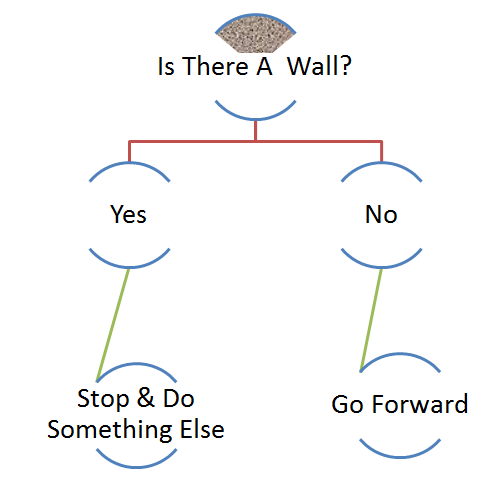
\includegraphics[height=0.4\textwidth]{imgk/salih-ifelse.png}
\end{center}
\vspace{-4mm}
\caption{This is how Karel uses the {\tt wall} sensor!}
\label{fig:dede-ifelse}
%\vspace{-10mm}
\end{figure}
\noindent
The usage of the {\tt wall} sensor in a program can be illustrated using a simple program "Careful step" 
where Karel first checks whether there is a wall ahead before
making a step. If there is wall, he turns back: 

\begin{bluecode}
# Program "Careful step".
if wall
    repeat 2
        left
else
    go
\end{bluecode}
As we mentioned before, the symbol '{\tt \#}' introduces a comment, meaning that the line 
of code behind it is ignored by the robot.
The {\tt else} branch does not have to be there if it is not needed. Notice the indentation 
of the bodies of the {\tt if} and {\tt else} branches - this is analogous 
to how we indent the body of the {\tt repeat} command. There are four more sensors:\\

\noindent
\underline{{\tt gem} sensor} returns true if the robot stands on a gem, false otherwise. \\

\noindent
\underline{{\tt empty} sensor} returns true if the robot's bag with gems is empty, false otherwise. \\

\noindent
\underline{{\tt north} sensor} returns true if the robot is facing North, false otherwise.\\

\noindent
\underline{{\tt home} sensor} returns true if the robot is at home, false otherwise.

\subsection*{Testing opposites}

Karel can also use the reserved word {\tt not} to test the opposites.
For illustration, the previous program can be rewritten as follows, without 
changing its function:
\begin{bluecode}
# Program "Careful step".
if not wall
    go
else
    repeat 2
        left
\end{bluecode}

\subsection{Programming hints}

Good programmer is a careful programmer! Errors can be avoided by always checking the 
appropriate sensor before making an action. A few examples of careful actions:
 
\begin{bluecode}
if not wall
    go
\end{bluecode}
Another example:
 
\begin{bluecode}
if gem
    get
\end{bluecode}
And a last one:
 
\begin{bluecode}
if not empty
    put
\end{bluecode}

%%%%%%%%%%%%%%%%%%%%%%%%%%%%%%%%%%%%%%%%%%%%%%%%%%%%%%%%%%%%%%%%%%%%%%%%%%%%%%%

\section{Conditional Loop} \label{sec:whilek}

\subsection{Objectives} 
 
\begin{itemize}
\item Learn to repeat a command or a sequence of commands when it is not known 
      how many repetitions will be needed.
\end{itemize}

\subsection{The {\tt while} command}

Often Karel needs to repeat something, {\em not knowing in advance how many repetitions
there will be}. So, the {\tt repeat} command is not practical. This can be the case, for example, 
when the robot is asked to walk straight ahead until he reaches the closest wall.
Remember that he only can see walls that are right ahead of him -- walls 
that are further away he can't see. Such a program would be:

\begin{bluecode}
while not wall
    go
\end{bluecode}
Or, Karel may be asked to walk until he gets home:

\begin{bluecode}
while not home
    go
\end{bluecode}
Beware though -- {\bf this program is dangerous} since the robot will crash into a wall
if his home is not straight ahead of him!

Another example: The robot may be asked to empty his bag (he does not know how many gems are in it): 
 
\begin{bluecode}
while not empty
    put
\end{bluecode}
Or, he may be asked to collect all gems from a pile (he does not know 
how many gems there are):

\begin{bluecode}
while gem
    get
\end{bluecode}
Or we may ask him to turn to face North (he does not know which direction he is
facing):

\begin{bluecode}
while not north
    left
\end{bluecode}
At last, let us face the following situation: Karel is asked to 
turn South, walk straight ahead until he reaches the closest wall, and 
collect all gems that he can find on the way:

\begin{bluecode}
# First turn North.
while not north
    left

# Then turn South.
repeat 2
    left

# Go straight ahead and pick all gems.
while not wall
    if gem
        get
    go

# Pick gem at the wall (if any).
if gem
    get
\end{bluecode}
Notice that we first need to turn the robot to face North -- this is because North 
is the only direction that he can check!


%%%%%%%%%%%%%%%%%%%%%%%%%%%%%%%%%%%%%%%%%%%%%%%%%%%%%%%%%%%%%%%%%%%%%%%%%%%%%%%

\section{Custom Commands} \label{sec:newcom}

\subsection{Objectives} 
 
\begin{itemize}
\item Learn that replicating computer code is a very bad habit.
\item Learn that splitting the big task into smaller ones will simplify the solution a lot. 
\item Learn to bring more structure and clarity into our programs by introducing new commands.
\end{itemize}

\subsection{Programming hints}

{\em Always look for small tasks that can be solved independently of the big ones.
Solve the small tasks first, and you will see that the big ones get much simpler. The 
importance of what we just said cannot be stressed more.}\\

\noindent
The fact that you are reading this line of text proves that you are not 
a perfect programmer yet. A perfect programmer would be stuck forever 
in the previous three lines which are an infinite loop!

%\begin{figure}[!ht]
%\begin{center}
%
\includegraphics[width=0.2\textwidth]{imgk/smiley.png}
%\end{center}
%\vspace{-1cm}
%\end{figure}

\subsection{Never replicate computer code}

A new command should be defined whenever it becomes clear that the same 
action is repeated in the algorithm multiple times (yes, we talk about the algorithm,
not about the program). When we start writing a program and then realize that the same
code repeats itself at various places, then probably we did not do a good job 
designing the algorithm.

Sometimes it might be 
tempting to just replicate the same code several times in the 
program, because it does the same thing, but do not do it! This would be very bad programming
and sooner or later our own code would punish us for that. 
We would make a small change at one place but forget to do it 
in all the other places. Then our code would start 
acting strange, it would sometimes work and sometimes fail. 
We would spend lots of time looking for the mistakes, find some 
of them but not all, and our program would become unreliable
and after some time irreparable. We would find that we need to 
rewrite it from scratch.

\subsection{Defining new commands}

New commands are defined using the reserved word 
{\tt def}. For example, in a program where the robot needs to turn back
many times, it is a good idea to define a new command {\tt back}
as follows:

\begin{bluecode}
def back
    repeat 2
        left
\end{bluecode}
Note the indent -- the body of a new command needs to be indented 
analogously to the bodies of loops and conditions.

%%%%%%%%%%%%%%%%%%%%%%%%%%%%%%%%%%%%%%%%%%%%%%%%%%%%%%%%%%%%%%%%%%%%%%%%%%%%%%%

\section{Recursion} \label{sec:recursion}

\subsection{Objectives} 
 
\begin{itemize}
\item Understand what recursion is and when it can be useful.
\item Learn to write good recursive algorithms.
\end{itemize}
By a {\em recursive} algorithm we mean an algorithm that uses itself. Doesn't it sound weird?
But in our life we use recursion all the time, for example when we descend a staircase.
With a bit of abstraction, our algorithm is:

\begin{bluecode}
Descend_staircase
    Descend one step
    If this was not the last step
        Descend_staircase
\end{bluecode}
Recursion is not advantageous for all types of problems, but it can be really 
helpful, especially for problems where 
\begin{itemize}
\item we can do some work to reduce the problem to the same one but smaller in size, 
\item we can apply the same algorithm to the smaller problem. 
\end{itemize}
On program level, this means that some command calls itself, either 
directly or through other commands.

\subsection{How it works} 

Consider the following program:
\begin{bluecode}
def reach_wall
    if not wall
        go
        reach_wall

reach_wall
\end{bluecode}
\noindent
Imagine that the initial position of the robot is like in Fig. \ref{fig:rec1}.


\begin{figure}[!ht]
\begin{center}
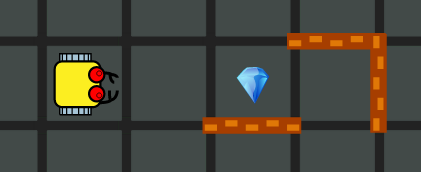
\includegraphics[width=6cm]{imgk/rec-1.png}
\end{center}
\vspace{-4mm}
\caption{Robot's initial position.}
\label{fig:rec1}
\vspace{-4mm}
\end{figure}
\noindent
When the command {\tt reach\_wall} is first called, the robot stands three steps away from the wall and 
thus the {\tt if not wall} condition passes. Then the command {\tt go} follows and the robot's 
position changes as shown in Fig. \ref{fig:rec2}. 
\newpage

\begin{figure}[!ht]
\begin{center}
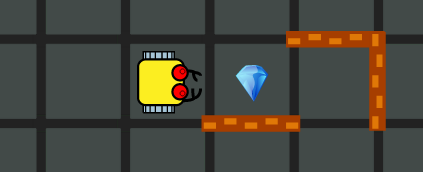
\includegraphics[width=6cm]{imgk/rec-2.png}
\end{center}
\vspace{-4mm}
\caption{Robot's position after the first {\tt if not wall} condition passes and he makes the first step forward.}
\label{fig:rec2}
\vspace{-4mm}
\end{figure}
\noindent
Next the robot executes the {\tt reach\_wall} command that follows the {\tt go} command. A good way to 
understand what happens is to imagine that the command is replaced with its own body. The corresponding 
program would look as follows:

\begin{bluecode}
if not wall
    go
    if not wall
        go
        reach_wall
\end{bluecode}
\noindent
Since the robot is two steps away from the wall, the second {\tt if not wall} condition passes and 
he makes a second step forward. His new position is shown in Fig. \ref{fig:rec3}.

\begin{figure}[!ht]
\begin{center}
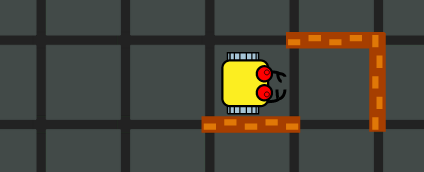
\includegraphics[width=6cm]{imgk/rec-3.png}
\end{center}
\vspace{-4mm}
\caption{Robot's position after the second {\tt if not wall} condition passes and he makes a second step forward.}
\label{fig:rec3}
\vspace{-4mm}
\end{figure}
\noindent
Next the robot executes the third {\tt reach\_wall} command. Again we can imagine that the command 
is replaced with its own body. The corresponding program would look as follows:

\begin{bluecode}
if not wall
    go
    if not wall
        go
        if not wall
            go
            reach_wall
\end{bluecode}
\noindent
Since the robot is one step away from the wall, the third {\tt if not wall} condition passes and 
he makes a third step forward. His new position is shown in Fig. \ref{fig:rec4}.

\begin{figure}[!ht]
\begin{center}
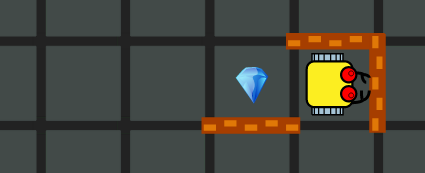
\includegraphics[width=6cm]{imgk/rec-4.png}
\end{center}
\vspace{-4mm}
\caption{Robot's position after the third {\tt if not wall} condition passes and he makes a third step forward.}
\label{fig:rec4}
%\vspace{-10mm}
\end{figure}
\noindent
Next the robot executes the {\tt reach\_wall} command again and we can imagine that the command 
is replaced with its own body. The corresponding program would look as follows:

\begin{bluecode}
if not wall
    go
    if not wall
        go
        if not wall
            go
            if not wall
                go
                reach_wall
\end{bluecode}
\noindent
However, now the robot is facing the wall and thus the {\tt if not wall} condition does not pass.  
This means that the program is finished!

\subsection{The base case}

In the previous example we have seen one important fact: To prevent infinite recursion, one always needs {\tt if} or {\tt if-else} 
statement of some sort where one branch makes a recursive call, and the other branch is either 
missing or it does not make a recursive call. The branch without a recursive 
call is called the {\em base case}. A bad example of a recursive command without a base case would be 

\begin{bluecode}
def left_forever
    left
    left_forever
\end{bluecode}
\noindent
One can guess where the name of this command comes from! Fortunately, the program can be stopped using 
either the red button or the {\tt stop} button under the code cell.

\subsection{When should recursion be used?}

The recursive command {\tt reach\_wall} that we defined above may not be the most useful example 
since the same functionality could be achieved more elegantly without recursion, just with

\begin{bluecode}
def reach_wall
    while not wall
        go
\end{bluecode}
If there is a small task that needs to be solved repeatedly in order to get a bigger task done,
then often one can write both a non-recursive and a recursive algorithm. Recall for example the Diamond
Staircase example from Section \ref{sec:newcom}. The small task there was to climb one step and pick 
up the gem, ending up facing east. The non-recursive version of the algorithm would be:

\begin{bluecode}
def climb_one_step
    left
    go
    right
    go
    get

while not home
    climb_one_step
\end{bluecode}
The recursive version of the algorithm looks as follows:

\begin{bluecode}
def climb_the_stairs
    if not home
        left
        go
        right
        go
        get
        climb_the_stairs

climb_the_stairs
\end{bluecode}
If it is easy to write a non-recursive version of an algorithm, then it should be used
because in general, non-recursive algorithms are faster. 
Recursive version of an algorithm should be used if a non-recursive version would 
be difficult to design. For example, nearly all code written for tree-like structures 
is recursive. Also many sorting algorithms are more naturally written in recursive form.
We will come to these subjects later.

\subsection{Mutually recursive commands}

Recursion can have interesting forms. In its simplest shape, a command 
calls itself in its own body. But, we can have a pair of commands
that call themselves mutually, such as the commands {\tt odd} and 
{\tt even} in the following example (that also solves the Diamond Staircase
problem by the way):
 
\begin{bluecode}
def climb_step
    left
    go
    right
    go
    get 

def odd
    if not home
        climb_step
        even
    
def even
    if not home
        climb_step
        odd
    
odd
\end{bluecode}
Obviously this program is not the most efficient one to solve the 
Diamond Staircase problem, but it is great for illustration purposes.

%%%%%%%%%%%%%%%%%%%%%%%%%%%%%%%%%%%%%%%%%%%%%%%%%%%%%%%%%%%%%%%%%%%%%%%%%%%%%%%

\section{Variables and Lists} \label{sec:var}

In this Section we are entering exciting Level 3! Karel grew up and left the home of his 
parents to experience a life of his own. Therefore, his home will not be present
in the following exercises and games anymore. There are a few more changes
that reflect Karel's growing up, including numerical and logical variables,
functions that return values, and lists. Do not forget to adjust the level 
to Level 3 in Settings. A compact overview of new functionality in Level 3 
can be found in Section \ref{sec:newfunc3}.

\subsection{Objectives} 
 
\begin{itemize}
\item Understand the concept of variables.
\item Learn to work with numerical and logical variables.
\item Learn to use functions that return values. 
\item Understand that variables defined inside functions are local. 
\item Learn to work with lists.
\end{itemize}

\noindent
In programming, variables are used to store useful information for later use. This information can 
be a number, word, sentence, or anything else. 

\subsection{Types of variables}

All of us are using variables in our lives. One of 
the first ones is our own name. With a bit of abstraction (and say that your name is "Melissa"), 
when you were about two years old, you did the following:

\begin{bluecode}
my_name = "Melissa"
\end{bluecode}
Since then, each time someone called a name, you retrieved in your brain the value of the variable
{\tt my\_name}, compared it to the name that you heard, and if you got a match then you turned around 
to see who was calling you. Imagine that we would not be able to use that variable!

The variable {\tt my\_name} stores a word (string of characters). We also use many numerical variables such as
{\tt seconds\_per\_minute} whose value is 60, {\tt minutes\_per\_hour} whose value is 60 as well, 
{\tt hours\_per\_day} whose value is 24, and we could go on. The last three variables do not change 
too often, most likely they will not change during our lives. But we also use variables whose 
values change, such as {\tt days\_per\_year}, {\tt number\_of\_my\_pets}, etc. In Karel, we
will only use integer numbers.

Next let's look at logical variables. Those are variables that only can store two possible values --
{\tt True} or {\tt False}, and we use a huge number of them. One such example may be {\tt I\_speak\_a\_foreign\_language}.
For someone this variable has the value {\tt False}, for someone it is {\tt True}. The important 
thing is that when someone asks you about that, you do not need to go check the records in the language 
school -- you just know it. The value is {\em stored}, it does not have to be {\em created} each time 
it is needed. Logical variables will be discussed in more detail shortly -- first let us explore 
the numerical ones.

\subsection{Reading GPS coordinates}

Karel's coolest Christmas present was a new GPS device that allows him to determine his position 
in the maze. With it, he will never get lost again! He can retrieve his coordinates at any time via the 
kaywords {\tt gpsx} and {\tt gpsy}. He also has a new ability to output results via the {\tt print} 
command. The usage of these commands is best illustrated using the following short program where 
Karel determines his coordinates in the maze and prints them:

\begin{bluecode}
print "Horizontal position:", gpsx
print "Vertical position:", gpsy
\end{bluecode}
The south-west corner of the maze is the origin of the coordinate system and it has 
coordinates [0, 0]. Let's say that Karel stands as shown in Fig. \ref{fig:gps-100}.

\begin{figure}[!ht]
\begin{center}
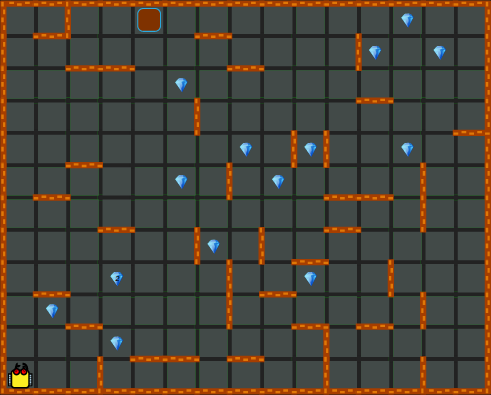
\includegraphics[height=0.4\textwidth]{imgk/gps-100.png}
\vspace{-0mm}
\caption{South-west corner of the maze has GPS coordinates [0, 0].}
%\vspace{-1cm}
\label{fig:gps-100}
\end{center}
\end{figure}
\noindent
Then the above program has the following output:

\begin{bluecode}
Horizontal position: 0
Vertical position: 0
\end{bluecode}
The maze's width (in west-east direction) is 15 tiles, and its height (in south-north direction) 
is 12 tiles. If Karel stands in the north-east corner as shown in Fig. \ref{fig:gps-101},

\begin{figure}[!ht]
\begin{center}
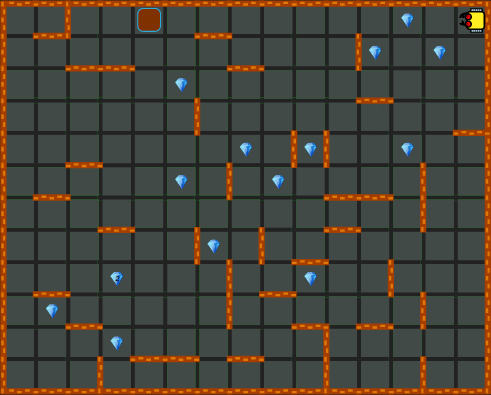
\includegraphics[height=0.4\textwidth]{imgk/gps-101.png}
\vspace{-0mm}
\caption{North-east corner of the maze has GPS coordinates [14, 11].}
%\vspace{-1cm}
\label{fig:gps-101}
\end{center}
\end{figure}
\newpage
\noindent
then the output of the program is

\begin{bluecode}
Horizontal position: 14
Vertical position: 11
\end{bluecode}
Try it! Also move Karel to other parts of the maze in Designer and run the program again
to make yourself familiar with how the GPS device works.

\subsection{Custom Functions}

In Level 3 we can use the reserved word {\tt return} inside the body of
a command to return a value. Such commands are then called {\em functions}. 
They are also defined using the keyword {\tt def}. For example, the following function
{\tt count\_steps} will return the number of steps the robot needed to 
make in order to reach the closest wall in the direction that he was facing:

\begin{bluecode}
def count_steps
    n = 0
    while not wall
        go
        inc(n)
    return n
\end{bluecode}
The function can be then used as follows:

\begin{bluecode}
num = count_steps
print "Number of steps:", num 
\end{bluecode}

\subsection{Creating numerical variables} \label{par:var}

In Karel, numerical variables can be created in several different ways: 
\begin{enumerate}
\item By setting them to an integer number. For example, new variable {\tt a} is created and set to zero by typing 
\begin{bluecode}
a = 0
\end{bluecode}
\item By setting them to {\tt gpsx}. For example, new variable {\tt var} is created and set to {\tt gpsx} by typing
\begin{bluecode}
var = gpsx
\end{bluecode}
\item By setting them to {\tt gpsy}. For example, new variable {\tt pos1} is created and set to {\tt gpsy} by typing
\begin{bluecode}
pos1 = gpsy
\end{bluecode}
\item Initialize them with an existing value. For example, if we already have a variable {\tt var1}, then a new variable 
{\tt var2} can be created as follows:
\begin{bluecode}
var2 = var1
\end{bluecode}
\item Initialize them with value returned by an existing function, as it was shown in the previous 
paragraph. 
\end{enumerate}

\subsection{Changing values of numerical variables}

The value of a numerical variable can be updated at any time by redefining it via 
one of the four options described in the previous paragraph. For example, let's say that 
Karel stands as shown in Fig. \ref{fig:var1}.
\begin{figure}[!ht]
\begin{center}
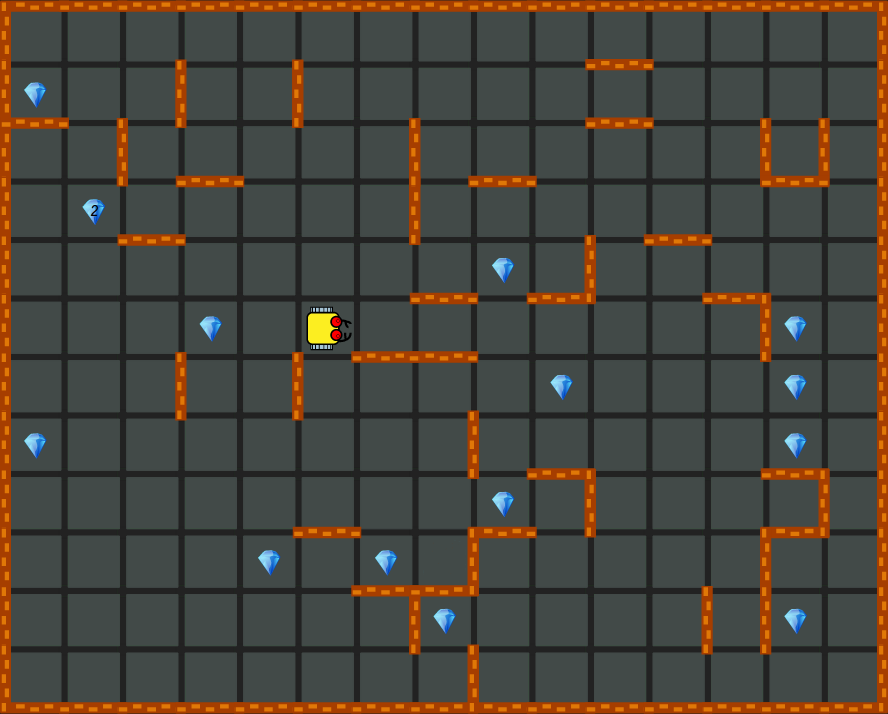
\includegraphics[height=0.4\textwidth]{imgk/variables1.png}
\end{center}
\vspace{-4mm}
\caption{Karel's initial position.}
\label{fig:var1}
%\vspace{-1cm}
\end{figure}

\noindent
Then the program

\begin{bluecode}
a = gpsx
print "Start position:", a
repeat 5
    go
a = gpsx 
print "End position:", a
\end{bluecode}
will produce the following output:

\begin{bluecode}
Start position: 5
End position: 10
\end{bluecode}
Another way to change the value of a numerical variable is to increase it by one or 
decrease it by one via the commands {\tt inc()} and 
{\tt dec()}, respectively. Commands {\tt inc(a, num)} and 
{\tt dec(a, num)} will increase / decrease the value of variable {\tt a}
by an integer number {\tt num}.

Consider again Karel's initial position as shown 
in Fig. \ref{fig:var1}. Then the code

\begin{bluecode}
a = zero
while not wall
    go
    inc(a)
print "Went", a, "steps before reaching a wall."
\end{bluecode}
will have the following output:

\begin{bluecode}
Went 7 steps before reaching a wall.
\end{bluecode}

\subsection{Comparison operations}

Integer numbers and numerical variables can be compared using the 
standard operators {\tt >, <, >=, <=, ==, !=, <>}. In this order, 
they read "greater than", "less than", "greater than or equal to", 
"less than or equal to", "equal to", "not equal to" and "not equal to"
(the last two operations have the same meaning). The result of each such 
operation is a logical value {\tt true} or {\tt false}, and it can be 
either used in a condition or conditional loop, or assigned to 
a variable. For example,

\begin{bluecode}
a = 1
b = 5
print a < b
\end{bluecode}
yields the output

\begin{bluecode}
True
\end{bluecode}
The code

\begin{bluecode}
a = 1
b = 5
c = a > b
print c
\end{bluecode}
yields

\begin{bluecode}
False
\end{bluecode}
The code 

\begin{bluecode}
a = 0
while a <= 5
  print a 
  inc(a)
\end{bluecode}
yields 

\begin{bluecode}
0
1
2
3
4
5
\end{bluecode}

\subsection{Lists}

Lists are extremely useful data structures that can be used to store multiple 
objects in one variable at the same time. 
Such as, for example, integer variables, text strings, and even other lists.
Objects in a list are ordered and they can be added to the end of a list 
using the {\tt append()} function, accessed by their index, and 
deleted via the {\tt pop()} function or the {\tt del} command. Let us 
illustrate their usage on examples.\\

\noindent
\underline{\em Creating a list}\\

An empty list {\tt U} is created via 

\begin{bluecode}
U = []
\end{bluecode}
Lists can be also created non-empty:

\begin{bluecode}
V = [1, 2, 3, 4, 5]
\end{bluecode}
One can use variables when creating a list, as can be 
illustrated using the code

\begin{bluecode}
c = 100
W = [0, 50, c]
print W
\end{bluecode}
whose output is 

\begin{bluecode}
[0, 50, 100]
\end{bluecode}
Integer numbers can be combined with strings:

\begin{bluecode}
X = [1, "Hello", 2]
\end{bluecode}
Lists can contain other lists as their elements:

\begin{bluecode}
Y = [1, "Hello", 2, [1, 2, 3]]
\end{bluecode}
One can print a list as expected:

\begin{bluecode}
print "This is the list Y:", Y
\end{bluecode}
Output:

\begin{bluecode}
This is the list Y: [1, "Hello", 2, [1, 2, 3]]
\end{bluecode}
\underline{\em Accessing list items by indices}\\

Any list item can be accessed and either printed, assigned 
to a variable, or used in an operation, via its index. It is important to remember that 
the indices start from zero. In other words, {\tt L[0]} is the 
first item in the list, {\tt L[1]} is the second one, etc. For
illustration, let us show a sample code

\begin{bluecode}
G = [8, 12, 16, 20]
print "First item:", L[0]
print "Second item:", L[1]
print "Third item:", L[2]
print "Fourth item:", L[3]
\end{bluecode}
whose output is

\begin{bluecode}
First item: 8
Second item: 12
Third item: 16
Fourth item: 20
\end{bluecode}
\underline{\em Appending items to a list}\\

An arbitrary integer number, text string, or another list {\tt obj} can be appended 
to the end of an existing list {\tt L} as follows:

\begin{bluecode}
L.append(obj)
\end{bluecode}
This can be illustrated using the code

\begin{bluecode}
L = [1, 11]
L.append(21)
print L
\end{bluecode}
whose output is 

\begin{bluecode}
[1, 11, 21]
\end{bluecode}
\underline{\em Removing items via the {\tt pop()} function}\\

The {\tt i}-th item can be deleted from a list {\tt L} 
and assigned to a variable {\tt x} via 

\begin{bluecode}
x = L.pop(i)
\end{bluecode}
Recall that indices start from zero. The usage can be illustrated using the code

\begin{bluecode}
L = ["Monday", "Tuesday", "Wednesday"]
day = L.pop(1)
print day
print L
\end{bluecode}
whose output is 

\begin{bluecode}
Tuesday
['Monday', 'Wednesday']
\end{bluecode}
If the {\tt pop()} function is used without an index, it removes
and returns the last object of the list.\\

\noindent
\underline{\em Deleting items via the {\tt del} command}\\

The purpose of the {\tt del} command is similar to the {\tt pop()} function
except that the deleted object is destroyed (it cannot be assigned to a variable).
The {\tt i}-th item can be deleted from a list {\tt L} via 

\begin{bluecode}
del L[i]
\end{bluecode}
For illustration, the output of the code 

\begin{bluecode}
L = ["Monday", "Tuesday", "Wednesday"]
del L[0]
print L
del L[0]
print L
\end{bluecode}
is 

\begin{bluecode}
['Tuesday', 'Wednesday']
['Wednesday']
\end{bluecode}
\underline{\em Length of a list}\\

One can use the function {\tt len(X)} to obtain the length of a list {\tt X} -- an integer
number that can in turn be used to parse the list via a {\tt repeat} command.
The following sample code defines a list {\tt M} consisting of four numbers 
{\tt 1, 2, 3} and {\tt 4} and prints all of them increased by two: 

\begin{bluecode}
M = [1, 3, 5, 7]
n = len(L)
i = 0
repeat n
    c = M[i]
    print inc(c, 2)
    inc(i)
\end{bluecode}
\underline{\em Storing the robot's path in a list}\\

Lists can be used to store the robot's path. The following 
is a simple program that only tells the robot to go straight to the 
nearest wall (this part does not really matter) and store the GPS
coordinates in a list {\tt L}:

\begin{bluecode}
L = []
while not wall
    L.append([gpsx, gpsy])
    go
L.append([gpsx, gpsy])
print "Path: ", L
\end{bluecode}
In fact, each time we are appending a list consisting of the horizontal and 
vertical GPS coordinates -- there is no other way to represent two numbers 
in one variable unless the variable is a list. When the robot's initial position 
is as shown in Fig. \ref{fig:list-1},

\begin{figure}[!ht]
\begin{center}
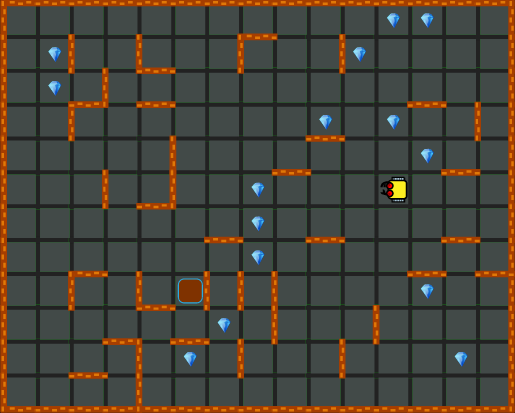
\includegraphics[height=0.4\textwidth]{imgk/lists-1.png}
\vspace{-0mm}
\caption{Robot stands at position [11, 6] facing west.}
%\vspace{-1cm}
\label{fig:list-1}
\end{center}
\end{figure}

\noindent
then the output of the above program is

\begin{bluecode}
Path: [[11, 6], [10, 6], [9, 6], [8, 6], [7, 6], [6, 6], [5, 6]]
\end{bluecode}
To keep Karel's language simple, we do not allow double indices. Nevertheless
there is a simple way to get to the items of lists that are contained in other lists:

\begin{bluecode}
a = L[0]
print "Horizontal coordinate of initial position:", a[0]
print "Vertical coordinate of initial position:", a[1]
a = L[1]
print "Horizontal coordinate after one step:", a[0]
print "Vertical coordinate after one step:", a[1]
...
\end{bluecode}

\subsection{Local and global variables}\label{subsec:karellocvar}

Note that a variable that is defined inside a function is {\em local to that function}, 
meaning that it can be used in the function only. If we attempt to use it 
outside, an error is thrown. For illustration, the code 

\begin{bluecode}
def myfunction
  a = 1

myfunction
print a  
\end{bluecode}
throws an error message 

\begin{bluecode}
Unknown variable/procedure "a" 
\end{bluecode}
Although using local variables might seem constraining, in reality it helps us 
to keep our code fit. It is a very good habit to keep variables in our programs 
as local as possible. More about local and global variables will be said in 
Part II, Subsection \ref{subsec:pythonlocvar}.

%%%%%%%%%%%%%%%%%%%%%%%%%%%%%%%%%%%%%%%%%%%%%%%%%%%%%%%%%%%%%%%%%%%%%%%%%%%%%%%

\section{Logic} \label{sec:logic}

\subsection{Objectives} 
 
\begin{itemize}
\item Learn to work with elementary and more complex logical expressions.
\end{itemize}

\subsection{Logical expressions}
As we already know, logical expressions are expressions that can be answered with either {\tt True} or 
{\tt False}. We say that the {\tt True} or the {\tt False} is their value. Here are some 
real-life examples, try to answer them with {\tt True} or {\tt False}:

\begin{itemize}
\item "I am 15 years old."
\item "My dad is a teacher."
\item "My school's name is Coral Academy."
\end{itemize}
And here are some Karel examples:
\begin{itemize}
\item wall ({\tt True} if the robot is facing a wall, {\tt False} otherwise)
\item home ({\tt True} if the robot is home, {\tt False} otherwise)
\item gem ({\tt True} if the robot stands on a gem, {\tt False} otherwise)
\item north ({\tt True} if the robot is facing North, {\tt False} otherwise)
\item empty ({\tt True} if the robot does not have any gems on him, {\tt False} otherwise)
\end{itemize}

\subsection{Logical variables}

In programming as well as in real life we often deal with logical expressions that are 
fairly complex. Often we use two or more simple logical expressions in one sentence, 
and moreover combine them with logical operations {\em and}, {\em or} or {\em not}.

For example, the sentence "I will go skiing on Saturday if weather is good and if 
Michael goes as well." includes three simple logical expressions. Let's call 
them for brevity\\

\noindent
A = "I will go skiing on Saturday."\\
B = "The weather is good."\\
C = "Michael goes as well."\\

\noindent
There is a logical operation {\em and} between the expressions B and C.

The original sentence can be written briefly as "if (B and C) then A". We love this kind of 
brevity in programming! A, B and C are {\em logical variables}. Logical variables 
can only represent {\tt True} or {\tt False}, and their purpose is to ease the operation with 
longer expressions.
Regarding the original sentence, we could go one step further and define a new logical variable\\

\noindent
D = B {\em and} C.\\

\noindent
Then, the sentence would become just "if D then A"! 

\subsection{Logical operations}

It is worth mentioning the following properties of the logical operation {\em and}:\\

\begin{center}
\framebox{(A {\em and} B) is {\tt True} only if both A and B are {\tt True}. Otherwise A {\em and} B is {\tt False}.}
\end{center}
\vspace{4mm}
\noindent
The logical operation {\em or} has the following properties:\\

\begin{center}
\framebox{(A {\em or} B) is {\tt True} if at least one of A, B is {\tt True}. If both A. B are {\tt False}, (A {\em or} B) is {\tt False}.}
\end{center}
\vspace{4mm}
\noindent
We also use the logical operation {\em not} with the following property:\\

\begin{center}
\framebox{({\em not} A) is {\tt True} if A is {\tt False} and vice versa.}
\end{center}

%%%%%%%%%%%%%%%%%%%%%%%%%%%%%%%%%%%%%%%%%%%%%%%%%%%%%%%%%%%%%%%%%%%%%%%%%%%%%%%

\section{Appendix - Overview of Functionality by Level}\label{sec:newfunc3}

\subsection{Level 0 (Section \ref{sec:manual})}

In Level 0, Karel can be guided by clicking on buttons:
\begin{itemize}
\item Go ... make one step forward.
\item Left ... turn left.
\item Right ... turn right.
\item Put ... put a gem on the ground.
\item Get ... pick up a gem from the ground.
\end{itemize}

\subsection{Level 1 (Section \ref{sec:bridge})}

In Level 1, Karel can be guided by typing the commands:
\begin{itemize}
\item {\tt go} ... make one step forward.
\item {\tt left} ... turn left.
\item {\tt right} ... turn right.
\item {\tt put} ... put a gem on the ground.
\item {\tt get} ... pick up a gem from the ground.
\end{itemize}

\subsection{Level 2 (Sections \ref{sec:repeat} -- \ref{sec:recursion})}

New commands:
\begin{itemize}
\item {\tt if - else} ... condition.
\item {\tt repeat} ... counting loop (repeat an action a given number of times).
\item {\tt while} ... conditional loop (repeat an action while a condition is satisfied).
\item {\tt def} ... define a new command.
\end{itemize}
Additional new keywords:
\begin{itemize}
\item {\tt wall} ... sensor that checks True if the robot faces a wall.
\item {\tt gem} ... sensor that checks True if there is a gem within the robot's reach.
\item {\tt empty} ... sensor that checks True if the robot's bag with gems is empty.
\item {\tt home} ... sensor that checks True if the robot is at home.
\item {\tt north} ... sensor that checks True if the robot faces North.
\end{itemize}
New functionality:
\begin{itemize}
\item Recursion (a command can make a call to itself).
\end{itemize}

\subsection{Level 3 (Sections \ref{sec:var}, \ref{sec:logic})}

New keywords:
\begin{itemize}
\item {\tt print} ... print strings and variables.
\item {\tt gpsx} ... GPS coordinate in the horizontal direction.
\item {\tt gpsy} ... GPS coordinate in the vertical direction.
\item {\tt a = 0} ... create a new variable {\tt a} and initialize it with zero (or another 
      integer number).\\ For additional ways to initialize variables see Subsection \ref{par:var}.
\item {\tt inc(a)} ... increases the value of variable {\tt a} by one.
\item {\tt inc(a, value)} ... increases the value of variable {\tt a} by {\tt value}.
\item {\tt dec(a)} ... decreases the value of variable {\tt a} by one.
\item {\tt dec(a, value)} ... decreases the value of variable {\tt a} by {\tt value}.
\item {\tt rand} ... random command (returns randomly True or False).
\item {\tt return} ... returns a value, to be used in functions.
\item {\tt and} ... binary logical {\em and}.
\item {\tt or} ... binary logical {\em or}.
\item {\tt not} ... unary logical {\em not}.
\item {\tt len(L)} ... length of list {\tt L}.
\item {\tt L[i]} ... object at position {\tt i} in list {\tt L}. Note: {\tt L[0]} is the first item in the list.
\item {\tt L.append(x)} ... appends {\tt x} to the end of list {\tt L}.
\item {\tt x = L.pop()} ... removes the last item of list {\tt L} and assigns it to {\tt x}.
\item {\tt del L[i]} ... removes from list {\tt L} object at position {\tt i}. 
\end{itemize}
New functionality:
\begin{itemize}
\item Numerical and logical (Boolean) variables.
\item Complex logical expressions.
\item Functions that return values.
\item Lists.
\end{itemize}
